\section{Analysis}
In the analysis the problem scope is defined by outlining the concept of the
application and with a more formal requirement list. 

\subsection{Application overview}
The application aims to make it easy for the users to create diagrams such as
\textit{UML} diagrams. Therefore the most basic functionality includes creating
classes and filling those out with fields and methods. To create a proper
diagram these classes should also be arranged and connected with different
relations such as inheritance or composistion. Since it is an editor, auxiliary
editing functionaliy such as deleting classes or relations and undo/redo is
of great importance. 

A few more advanced features is also important to consider. Saving and loading a
diagram allows the user to create a diagram and then commit changes at a later
point.

An user could use the produced diagram in a presentation or in a report by
taking a screenshot of the application, but a better approch would be to export
an image which could be directly embedded. Therefore an export feature would be
a great addition to the program. 

Since the amount of functions for the program is limited, an user interface
optimized for quickly selection the correct tool is also important. This also
includes hotkeys for the more proficient users. The original mockup from before
the development started can be seen in figure \ref{mockup}.
\begin{figure}[H]
\centering
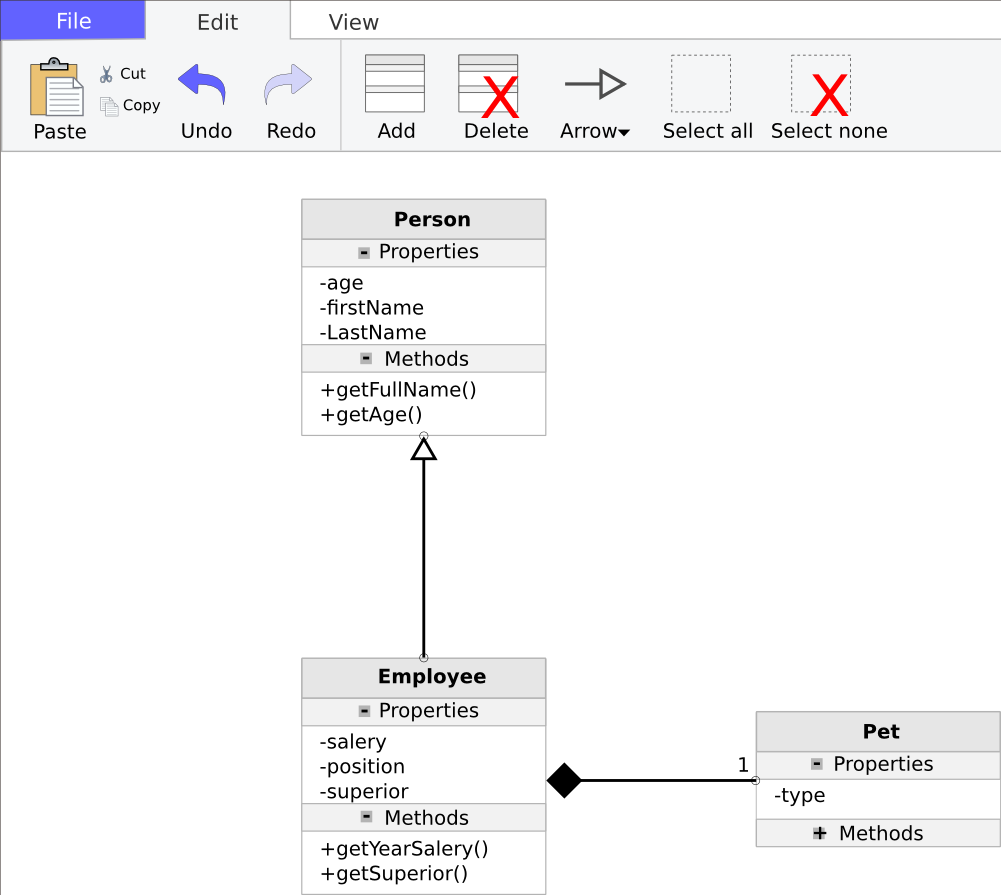
\includegraphics[width=\linewidth]{img/mockup}
\caption{Application mockup \label{mockup}}
\end{figure}

\subsection{Requirements}
Fill me in!!

